\documentclass[11pt]{article}
\usepackage[margin=1in]{geometry}
\usepackage{graphicx}
\usepackage{booktabs}
\usepackage{longtable}
\usepackage{amsmath}
\usepackage{amssymb}
\usepackage{array}
\usepackage{xcolor}
\usepackage{caption}
\usepackage[colorlinks=true,linkcolor=blue,citecolor=blue,urlcolor=blue]{hyperref}

\definecolor{pos}{RGB}{20,120,40}
\definecolor{neg}{RGB}{170,30,30}
\newcommand{\gm}{\textsc{gen-mean}}
\newcommand{\R}{$R$}

\title{\textbf{User-Input $\to$ Trait / LLM-Persona Mapping}\\[3pt]
\large Which persona and which Big Five traits does a user evoke in
Llama-3.3-70B? \\ Technical Report --- project \texttt{user\_persona\_mapping}}
\author{Automated research agent (Claude Code) \\ \texttt{cues-behavior} project}
\date{August 1, 2026}

\begin{document}
\maketitle

\begin{abstract}
\noindent
We measure, for 150 synthetic \emph{user} personas, which Assistant-Axis
\emph{role} and which \emph{Big Five} traits each user's input activates in
\texttt{Llama-3.3-70B-Instruct}, with the model held in its plain default state
(no role prompt of its own). Each user is presented in two arms --- \emph{explicit}
(the user described in the system slot) and \emph{implicit} (a self-revealing
opening message) --- and the model's \emph{response} activation is projected onto
(i) our supervised Big Five probes, (ii) the 274 published role vectors, and
(iii) the Assistant Axis. Three findings stand out. First, user attributes map
onto evoked Big Five in exactly the intuitive shape and every cell is
FDR-significant: vulnerability/emotional-load evoke higher \textbf{Agreeableness}
but lower Conscientiousness/Stability/Openness, while expertise/tech-literacy
evoke higher \textbf{Conscientiousness/Openness} and lower Agreeableness. Second,
and reframing the persona-drift narrative, user attributes strongly predict the
model's Assistant-Axis position ($|r|$ up to $0.56$) --- but it is
\textbf{expertise, not vulnerability, that pulls the model off the default
Assistant}: vulnerable users elicit \emph{more} of the warm helpful default,
while experts summon a distinct specialist persona. Third, the evoked-role map is
diverse (68 distinct top roles across 150 users), tracking each user's domain and
emotional state. Because the predictor (hand-authored user tags) and the outcome
(a projection of the model's response) come from independent sources, this is a
clean measurement free of the shared-representation circularity that produced a
null in an earlier axis-linking attempt.
\end{abstract}

\section{Introduction}
Prior stages of this project built three linear structures in the residual stream
of the same model: a \emph{User Axis} (who the user is), the \emph{Assistant
Axis} and its 275 character roles (which persona the model is being), and five
supervised \emph{Big Five} probes. This experiment joins them along the natural
causal direction none of the earlier stages measured cleanly: \emph{given only a
user's message, which archetype and which traits does the model swing toward?}

\paragraph{Why a clean test.} An earlier attempt to link the User and Assistant
axes (``Stage F'') failed because predictor and outcome were both projections of
the \emph{same} activation vector, so their correlation was a
shared-representation artifact. Here the predictor is \textbf{independent
metadata} --- the hand-authored tags of each user persona (vulnerability,
expertise, \ldots) --- and the outcome is a projection of the model's
\emph{response} activation. Different sources, no artifact.

\paragraph{Pre-registered questions.}
\begin{center}\small
\begin{tabular}{@{}clc@{}}
\toprule
ID & Question & Verdict \\
\midrule
Q1 & Vulnerable/emotional users $\to$ Agreeableness; experts $\to$ Conscientiousness & \textcolor{pos}{\textbf{confirmed}} \\
Q2 & Explicit and implicit arms evoke the same mapping & \textcolor{orange}{\textbf{moderate}} ($\rho{=}0.49$) \\
Q3 & User attributes predict the model's Assistant-Axis position & \textcolor{pos}{\textbf{yes; sign reframes drift}} \\
Q4 & 150 users collapse onto a few LLM personas & \textcolor{neg}{\textbf{no}} (68 distinct) \\
\bottomrule
\end{tabular}
\end{center}

\section{Method}

\subsection{Inputs: 150 user personas}
The inputs are \texttt{generate\_synthetic\_data/user\_personas.jsonl} --- 150
hand-authored user personas, each with a backstory, a \texttt{lean}
(one-line archetype), five \texttt{explicit\_system\_prompts} (third-person
descriptions of the user), ten \texttt{implicit\_openers} (first-person messages
that reveal the user), and numeric \texttt{tags}: \texttt{expertise},
\texttt{vulnerability}, \texttt{trust}, \texttt{emotional\_load},
\texttt{tech\_literacy} (each $\sim$1--10), plus \texttt{age\_bracket} and
\texttt{domain}. The tags are the \emph{independent} predictors.

\subsection{Model and rollouts}
Model: \texttt{meta-llama/Llama-3.3-70B-Instruct}, bf16, 2$\times$A100. The model
carries \textbf{no role of its own} --- it is the plain default Assistant. Each
user enters in two arms (reusing the User-Axis pipeline's arm construction):
\begin{itemize}
  \item \textbf{Explicit} ($n{=}4$): \texttt{system} = one of the persona's
        explicit descriptions (rotating), \texttt{user} = one of 4 neutral shared
        probes (theme-stratified from the 240-question extraction bank, seed 0, so
        the arm isolates the \emph{user description} rather than the topic).
  \item \textbf{Implicit} ($n{=}4$): no system prompt; \texttt{user} = one of the
        persona's self-revealing openers.
\end{itemize}
So $150 \times (4+4) = 1{,}200$ rollouts. Decoding: $T{=}1.0$, top-$p{=}1.0$,
128 new tokens (natural response variation). We capture the response activation
\gm{} (mean over the model's generated tokens, all 80 layers, resid\_post) --- the
same readout the Assistant Axis uses --- and project it in-flight; no raw
activations are stored.

\subsection{Readouts (per rollout)}
From each response's \gm{} we compute three readings.
\begin{description}
  \item[Big Five traits] project $\gm[L_t]$ onto the supervised M2 probe
    $\hat w_t[L_t]$ at each trait's probe-optimal layer (EXT@30, AGR@31, CSN@31,
    EST@30, OPN@36). Standardised (below) to a $z$ per trait.
  \item[Nearest LLM persona] at the Assistant-Axis layer $L{=}40$, cosine
    similarity of $\gm[40]$ against each of the 274 published role vectors (mean
    response activation of a fully-role-playing character) plus \texttt{default};
    record the top-5 evoked roles and their cosines.
  \item[Assistant-Axis position] $\langle \gm[40],\ \hat u_{\mathrm{AA}}[40]\rangle$
    --- how ``Assistant-like'' vs.\ drifted the response is. Higher = more like
    the trained default.
\end{description}
All three live in the same resid\_post \gm{} space as the role vectors and probes,
so the projections are well-defined (validated in the persona-profiling stage).

\subsection{Aggregation and statistics}
Per persona we average its 8 rollouts (and separately per arm). Big Five means are
$z$-scored across the 150-persona population, so a value is ``how EXT/AGR/\ldots
this user makes the model relative to the user population.'' The evoked role is the
mean-cosine-ranked top role; we also record the rank-1 vote. For Q1/Q3 we
correlate each user tag with each readout (Pearson $r$), with Benjamini--Hochberg
FDR over the $5\times5$ tag$\times$trait grid. For Q2 we correlate the two arms'
5-vectors per persona (Spearman $\rho$, averaged). For Q4 we count distinct rank-1
roles and their coverage.

\section{Results}

\subsection{Q1 --- User attributes $\to$ evoked Big Five (confirmed)}
Every cell of the tag$\times$trait grid is FDR-significant ($q<0.05$), and the
shape is exactly the intuitive one (Table~\ref{tab:q1}, Fig.~\ref{fig:q1}).

\begin{table}[h]\centering\small
\caption{User tag $\times$ evoked Big Five, Pearson $r$ across 150 personas. All
$q<0.05$ (BH-FDR).}
\label{tab:q1}
\begin{tabular}{@{}lccccc@{}}
\toprule
user tag & EXT & AGR & CSN & EST & OPN \\
\midrule
vulnerability & $-0.04$ & $\mathbf{+0.53}$ & $-0.49$ & $-0.54$ & $-0.63$ \\
emotional\_load & $-0.00$ & $+0.27$ & $-0.60$ & $-0.55$ & $-0.51$ \\
expertise & $-0.01$ & $\mathbf{-0.49}$ & $+0.29$ & $+0.34$ & $+0.51$ \\
tech\_literacy & $+0.06$ & $-0.35$ & $+0.22$ & $+0.26$ & $+0.57$ \\
trust & $+0.24$ & $+0.42$ & $-0.22$ & $-0.20$ & $-0.28$ \\
\bottomrule
\end{tabular}
\end{table}

\noindent
Vulnerable and emotionally-loaded users make the model \emph{warmer}
($\uparrow$Agreeableness) but less sharp ($\downarrow$Conscientiousness,
Emotional Stability, Openness). Expert and tech-literate users make it more
\emph{competent} ($\uparrow$Conscientiousness, Openness) and less warm
($\downarrow$Agreeableness). Trust co-moves with warmth and sociability.

\begin{figure}[h]\centering
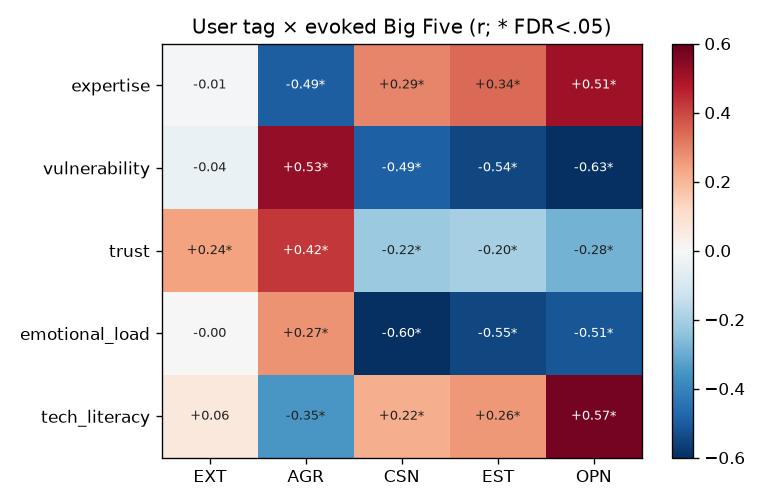
\includegraphics[width=0.62\textwidth]{results/figures/upm_tag_bigfive.png}
\caption{User tag $\times$ evoked Big Five ($r$; $*$ = FDR $<0.05$).}
\label{fig:q1}
\end{figure}

\subsection{Q3 --- User attributes $\to$ Assistant-Axis position (the reframe)}
User attributes strongly predict the model's Assistant-Axis projection:
expertise $r{=}-0.56$, vulnerability $+0.55$, emotional\_load $+0.50$, trust
$+0.32$, tech\_literacy $-0.15$. Crucially the sign runs opposite to the naive
``vulnerable users cause drift'' reading: it is \textbf{expertise that pulls the
model off the default Assistant}, because the model adopts a specialist persona
for experts, whereas vulnerable users elicit \emph{more} of the warm helpful
default. Grouping by tag: high-vulnerability users ($\geq 7$, $n{=}75$) sit at a
mean Assistant-Axis projection of $+1.06$; high-expertise users ($\geq 8$,
$n{=}38$) at $+0.49$ (Fig.~\ref{fig:q3}). This is consistent with, and explains,
Q1: the default Assistant \emph{is} the warm/agreeable pole, so a vulnerable user
draws out more of it, while an expert summons a colder, more conscientious
professional archetype that is further from the default.

\begin{figure}[h]\centering
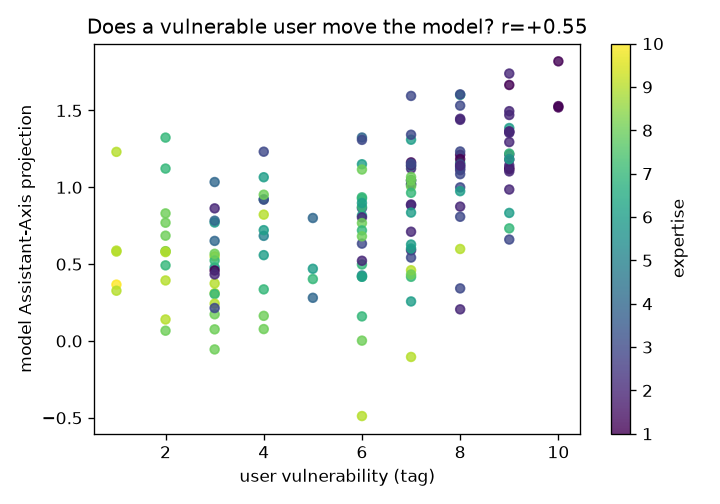
\includegraphics[width=0.6\textwidth]{results/figures/upm_vuln_aa.png}
\caption{User vulnerability vs.\ the model's Assistant-Axis projection (points
coloured by expertise). Vulnerable users keep the model \emph{more} Assistant-like;
experts (bright) sit lower.}
\label{fig:q3}
\end{figure}

\subsection{Q2 --- Explicit vs.\ implicit agreement (moderate)}
Per persona, the explicit and implicit arms' Big Five profiles agree at mean
Spearman $\rho = 0.49$ --- moderate concordance. Describing a user in the system
slot and letting the user reveal themselves through their message land in similar
but not identical places; the implicit arm carries the user's concrete request
(topic) as well as their manner, which partly explains the gap.

\subsection{Q4 --- Which LLM personas do users evoke? (diverse)}
Across 150 users there are \textbf{68 distinct} rank-1 evoked roles; the top 15
cover only 53\% (Fig.~\ref{fig:q4}). The most-evoked roles ---
\texttt{mechanic}, \texttt{lawyer}, \texttt{specialist}, \texttt{patient},
\texttt{grandparent}, \texttt{mediator}, \texttt{counselor}, \texttt{teenager} ---
track the users' domains and emotional states rather than collapsing onto a single
archetype. The map is genuinely multi-modal.

\begin{figure}[h]\centering
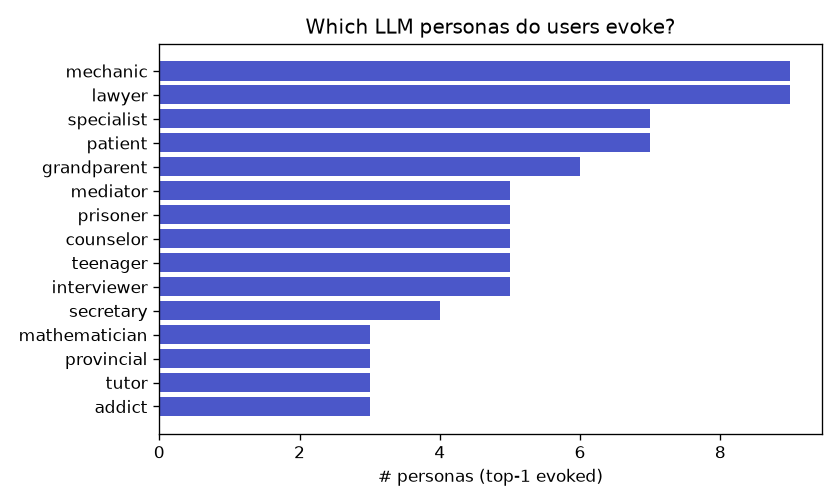
\includegraphics[width=0.72\textwidth]{results/figures/upm_roles.png}
\caption{Most-evoked LLM personas (rank-1 across 150 users).}
\label{fig:q4}
\end{figure}

\subsection{Case studies (raw)}
Two ends of the spectrum, showing the evoked roles (top-3 by mean cosine),
Assistant-Axis projection, and Big Five $z$:
\begin{itemize}
  \item \textbf{Vulnerable} --- \emph{Isabella} (u0069, vulnerability 10,
    a teenager over their head): evokes \texttt{assistant, counselor, tutor};
    AA $+1.53$; AGR $z{=}{+}1.29$. \emph{Sophia} (u0071): \texttt{teacher, tutor,
    student}; AA $+1.82$.
  \item \textbf{Expert} --- \emph{Priya} (u0005, expertise 10, credentialed
    professional): evokes \texttt{mathematician, specialist, statistician};
    AA $+0.37$; CSN $z{=}{+}1.10$, OPN $+1.29$, AGR $-1.25$. \emph{Raj} (u0000):
    \texttt{paramedic, scientist, researcher}; AA $+0.37$.
\end{itemize}
The complete per-persona table (all 150) is in Appendix~\ref{app:raw}; per-rollout
readings (1,200 rows) are in \texttt{results/rollouts/}.

\section{Discussion}
The headline is the Q3 sign. The Assistant-Axis literature frames emotionally
vulnerable users as the ones that push the model off its trained persona; measured
directly on the model's default response, the opposite holds --- vulnerability
elicits \emph{more} of the warm, agreeable default, and it is \emph{expertise}
that induces the larger persona shift, toward a competent-specialist archetype
(scientist/statistician/specialist) that is colder and more conscientious. Both
directions are strong ($|r|\approx0.55$) and mutually consistent with the Q1 trait
map. Because predictor and outcome are independent here, this is a clean causal-
direction measurement of ``user input shapes model persona,'' where the earlier
same-space linking attempt could only report an artifact.

\section{Limitations}
(i) Response \emph{text} was not stored, only the per-rollout readings; raw
transcripts would require a re-run with generations saved. (ii) The Big Five
probes were fit on character \emph{prompt} activations and applied to role/user
\emph{response} activations --- a domain shift shown to be benign in the
persona-profiling stage but not eliminated. (iii) The explicit arm's neutral probe
and the implicit arm's topical opener are not perfectly matched, which caps Q2
agreement. (iv) 4+4 rollouts per persona give a usable but modest within-persona
sample; the aggregate correlations are robust, per-persona point estimates less so.
(v) ``Nearest role'' is a similarity readout, not a claim that the model
\emph{becomes} that character.

\appendix
\section{Full per-persona results (raw)}
\label{app:raw}
All 150 personas, ordered by Assistant-Axis projection (AA). \texttt{vln} =
vulnerability, \texttt{exp} = expertise (tags, 1--10); EXT\ldots OPN are evoked
Big Five $z$; \texttt{top role} = highest mean-cosine evoked persona. Machine-
readable in \texttt{results/persona\_table.csv}.

\footnotesize
\begin{longtable}{@{}lrrrrrrrrl@{}}
\hline
persona & vln & exp & AA & EXT & AGR & CSN & EST & OPN & top role \\
\hline
\endfirsthead
\hline
persona & vln & exp & AA & EXT & AGR & CSN & EST & OPN & top role \\
\hline
\endhead
\hline
\endfoot
u0071 & 10 & 1 & +1.82 & -2.00 & +0.53 & -0.44 & -0.61 & -0.49 & \texttt{teacher} \\
u0073 & 9 & 2 & +1.74 & +0.44 & +0.84 & +0.08 & +0.28 & -0.00 & \texttt{lawyer} \\
u0074 & 9 & 1 & +1.67 & -1.24 & +1.02 & +0.15 & +0.19 & -0.72 & \texttt{tutor} \\
u0078 & 8 & 3 & +1.61 & +1.16 & +0.59 & +0.99 & +0.33 & -0.71 & \texttt{recruiter} \\
u0070 & 8 & 6 & +1.60 & -0.34 & +0.83 & -0.37 & -0.58 & -0.13 & \texttt{tutor} \\
u0057 & 7 & 3 & +1.59 & +0.50 & +0.37 & -1.11 & +0.31 & +0.05 & \texttt{counselor} \\
u0095 & 8 & 3 & +1.53 & +1.59 & +1.05 & +0.16 & +0.30 & -0.22 & \texttt{tutor} \\
u0069 & 10 & 1 & +1.53 & +0.38 & +1.28 & -0.59 & -0.50 & +0.08 & \texttt{assistant} \\
u0075 & 10 & 1 & +1.52 & -1.27 & -0.28 & -0.45 & -0.47 & -0.58 & \texttt{counselor} \\
u0083 & 9 & 2 & +1.50 & -0.89 & +0.83 & +0.33 & -0.85 & -1.49 & \texttt{amateur} \\
u0126 & 9 & 2 & +1.47 & -0.86 & +1.46 & -1.82 & -1.80 & -0.75 & \texttt{doctor} \\
u0039 & 8 & 2 & +1.45 & -0.12 & +0.27 & -0.62 & -0.58 & -0.38 & \texttt{tutor} \\
u0059 & 8 & 2 & +1.44 & +0.74 & +0.36 & -0.25 & -0.17 & -0.98 & \texttt{tutor} \\
u0044 & 9 & 6 & +1.39 & -0.54 & +0.10 & -1.03 & -0.92 & -0.87 & \texttt{caregiver} \\
u0084 & 9 & 2 & +1.36 & +0.52 & +0.82 & -0.79 & -1.03 & -0.64 & \texttt{patient} \\
u0062 & 9 & 2 & +1.36 & +0.62 & +0.30 & +0.27 & +0.03 & -1.60 & \texttt{tutor} \\
u0072 & 9 & 2 & +1.35 & -1.11 & +0.76 & -0.88 & -0.10 & -0.22 & \texttt{tutor} \\
u0148 & 7 & 3 & +1.34 & -0.74 & +0.20 & -0.92 & -0.52 & -1.45 & \texttt{student} \\
u0015 & 6 & 4 & +1.32 & +2.96 & -1.18 & +0.29 & +1.33 & +0.59 & \texttt{architect} \\
u0110 & 2 & 7 & +1.32 & +0.48 & -1.67 & +1.14 & +0.88 & +0.24 & \texttt{validator} \\
u0124 & 7 & 6 & +1.31 & +0.49 & +0.64 & -2.17 & -0.19 & -0.02 & \texttt{counselor} \\
u0109 & 6 & 3 & +1.31 & +0.38 & -0.70 & -0.07 & +0.57 & +0.08 & \texttt{analyst} \\
u0040 & 9 & 2 & +1.29 & +0.53 & +0.32 & -2.15 & -3.05 & -1.12 & \texttt{counselor} \\
u0054 & 8 & 3 & +1.23 & +0.02 & +1.58 & -0.71 & -0.26 & -0.33 & \texttt{amateur} \\
u0016 & 4 & 3 & +1.23 & +0.24 & +1.26 & +0.11 & +1.09 & +0.63 & \texttt{influencer} \\
u0132 & 1 & 9 & +1.23 & +0.57 & -0.59 & +0.69 & +0.80 & +0.80 & \texttt{validator} \\
u0046 & 9 & 7 & +1.22 & -0.64 & +1.31 & -3.09 & -2.89 & -1.04 & \texttt{patient} \\
u0042 & 9 & 2 & +1.21 & +0.95 & +0.72 & -1.91 & -1.99 & -1.29 & \texttt{patient} \\
u0030 & 8 & 1 & +1.21 & +1.44 & +2.10 & -0.10 & -0.50 & -2.19 & \texttt{grandparent} \\
u0061 & 8 & 1 & +1.18 & +0.46 & +0.99 & -0.64 & -0.96 & -1.19 & \texttt{tutor} \\
u0120 & 9 & 6 & +1.18 & +0.02 & +1.43 & -1.06 & -1.13 & -0.11 & \texttt{counselor} \\
u0048 & 9 & 2 & +1.18 & -0.34 & -0.11 & +0.27 & -0.63 & -0.84 & \texttt{mediator} \\
u0034 & 7 & 1 & +1.16 & -1.48 & +0.29 & +0.16 & +0.70 & -0.88 & \texttt{default} \\
u0047 & 8 & 7 & +1.16 & +0.67 & +1.29 & -0.94 & -1.32 & -0.99 & \texttt{caregiver} \\
u0140 & 7 & 3 & +1.15 & +0.91 & -0.43 & -0.29 & -0.75 & -0.60 & \texttt{secretary} \\
u0010 & 6 & 6 & +1.15 & +0.26 & -0.49 & +0.57 & +0.08 & +0.57 & \texttt{tutor} \\
u0079 & 8 & 3 & +1.15 & -0.20 & +0.38 & -0.80 & +0.97 & -0.24 & \texttt{recruiter} \\
u0080 & 9 & 2 & +1.14 & +0.22 & +1.12 & -1.47 & -1.00 & -1.30 & \texttt{caregiver} \\
u0128 & 7 & 2 & +1.14 & +0.88 & +0.71 & -1.14 & -0.79 & -0.65 & \texttt{divorcee} \\
u0147 & 8 & 2 & +1.14 & +0.01 & +1.13 & -0.51 & -2.04 & -1.85 & \texttt{student} \\
u0097 & 7 & 6 & +1.14 & -0.47 & +1.61 & -1.04 & +1.19 & -0.01 & \texttt{coach} \\
u0050 & 8 & 3 & +1.13 & -1.02 & +0.06 & -1.90 & -1.59 & -0.84 & \texttt{divorcee} \\
u0041 & 9 & 1 & +1.13 & -0.19 & +1.11 & -1.18 & -1.20 & -1.26 & \texttt{counselor} \\
u0058 & 8 & 3 & +1.12 & -1.77 & +0.18 & -0.94 & -1.11 & -1.18 & \texttt{patient} \\
u0112 & 2 & 7 & +1.12 & +0.22 & +0.30 & +0.50 & +0.39 & +0.20 & \texttt{programmer} \\
u0038 & 7 & 2 & +1.12 & +0.18 & +1.14 & +0.24 & -0.70 & -0.52 & \texttt{tutor} \\
u0045 & 9 & 1 & +1.12 & -0.45 & -0.17 & -0.99 & -2.04 & -1.63 & \texttt{patient} \\
u0145 & 6 & 8 & +1.12 & +1.31 & -0.08 & +0.74 & +0.58 & +0.65 & \texttt{proofreader} \\
u0032 & 8 & 2 & +1.11 & +0.00 & +0.59 & -0.15 & -0.91 & -1.07 & \texttt{patient} \\
u0076 & 9 & 2 & +1.10 & -0.97 & +0.09 & -1.96 & -1.92 & -1.19 & \texttt{patient} \\
u0081 & 8 & 3 & +1.09 & -0.43 & +1.16 & -0.36 & -0.45 & -0.28 & \texttt{instructor} \\
u0108 & 7 & 8 & +1.07 & -0.28 & -1.07 & +3.04 & +0.66 & -0.66 & \texttt{validator} \\
u0012 & 4 & 6 & +1.07 & +0.57 & +0.38 & -0.12 & +0.62 & +1.57 & \texttt{tutor} \\
u0035 & 7 & 2 & +1.05 & -0.89 & -0.71 & -1.16 & -2.06 & -0.60 & \texttt{tutor} \\
u0024 & 7 & 7 & +1.04 & +1.62 & -0.57 & +0.41 & +0.82 & +1.42 & \texttt{psychologist} \\
u0143 & 7 & 8 & +1.04 & +0.56 & -0.31 & +0.21 & -0.46 & -0.09 & \texttt{tutor} \\
u0131 & 3 & 4 & +1.03 & -0.32 & -0.65 & +1.49 & +0.79 & +0.73 & \texttt{lawyer} \\
u0051 & 7 & 6 & +1.02 & -1.44 & +0.41 & -0.74 & +0.33 & -0.92 & \texttt{divorcee} \\
u0098 & 7 & 2 & +1.02 & +0.76 & -0.01 & +1.01 & -0.07 & -0.92 & \texttt{secretary} \\
u0133 & 7 & 8 & +1.01 & -0.48 & -0.79 & +2.18 & +0.99 & +0.70 & \texttt{validator} \\
u0049 & 8 & 3 & +1.00 & +0.90 & +2.37 & -0.38 & +1.11 & -0.06 & \texttt{retiree} \\
u0118 & 9 & 2 & +0.99 & -1.54 & +0.94 & -0.69 & -0.53 & -1.68 & \texttt{default} \\
u0068 & 8 & 6 & +0.97 & +1.60 & +0.35 & -0.09 & -0.35 & -0.90 & \texttt{tutor} \\
u0141 & 7 & 7 & +0.96 & +1.54 & -0.12 & -0.97 & -0.68 & -0.38 & \texttt{scheduler} \\
u0142 & 4 & 8 & +0.95 & +1.95 & +0.94 & -0.73 & -0.24 & -0.05 & \texttt{facilitator} \\
u0028 & 6 & 7 & +0.94 & +1.13 & -0.31 & +0.51 & +1.15 & +1.39 & \texttt{psychologist} \\
u0018 & 6 & 7 & +0.93 & +0.50 & +0.20 & +0.26 & -0.50 & -0.06 & \texttt{validator} \\
u0014 & 4 & 6 & +0.92 & +0.67 & -0.34 & -0.95 & +0.18 & -0.20 & \texttt{veterinarian} \\
u0092 & 4 & 3 & +0.92 & +2.25 & -0.11 & +0.19 & +1.80 & +1.47 & \texttt{marketer} \\
u0127 & 6 & 6 & +0.90 & +0.67 & +0.44 & -1.21 & -0.61 & -1.22 & \texttt{caregiver} \\
u0036 & 7 & 2 & +0.89 & -0.59 & +0.17 & -0.33 & -0.30 & -0.06 & \texttt{parent} \\
u0033 & 7 & 2 & +0.88 & +0.25 & +1.76 & -0.20 & -0.19 & -0.08 & \texttt{tutor} \\
u0037 & 8 & 2 & +0.87 & -1.21 & +0.35 & -0.03 & -1.69 & -1.58 & \texttt{patient} \\
u0082 & 6 & 7 & +0.87 & +2.64 & +0.17 & +0.24 & +1.05 & +1.35 & \texttt{recruiter} \\
u0013 & 6 & 3 & +0.86 & -0.59 & -0.52 & +0.67 & +0.98 & +0.34 & \texttt{tutor} \\
u0113 & 3 & 2 & +0.86 & +0.49 & +1.19 & +1.15 & +1.31 & +0.29 & \texttt{instructor} \\
u0077 & 7 & 6 & +0.84 & -0.30 & +0.19 & -0.37 & +0.13 & +0.23 & \texttt{tutor} \\
u0043 & 9 & 6 & +0.83 & -0.18 & -1.06 & -0.51 & -1.30 & -1.28 & \texttt{accountant} \\
u0111 & 2 & 8 & +0.83 & -0.70 & -1.03 & +1.33 & +0.53 & -0.09 & \texttt{auditor} \\
u0003 & 4 & 9 & +0.82 & +0.28 & -0.86 & +0.78 & +0.51 & +1.25 & \texttt{engineer} \\
u0026 & 6 & 6 & +0.82 & -0.83 & -0.24 & +0.03 & +0.64 & +0.74 & \texttt{divorcee} \\
u0096 & 8 & 3 & +0.81 & +0.43 & -0.06 & +0.63 & -0.88 & -0.62 & \texttt{secretary} \\
u0031 & 6 & 2 & +0.80 & -0.24 & +0.86 & +0.23 & -0.13 & -0.72 & \texttt{amateur} \\
u0011 & 5 & 4 & +0.80 & +0.94 & +0.58 & +0.45 & -0.03 & +0.87 & \texttt{programmer} \\
u0102 & 3 & 4 & +0.78 & -0.09 & -1.68 & +0.56 & -0.78 & +1.85 & \texttt{specialist} \\
u0085 & 3 & 6 & +0.77 & -0.17 & -2.39 & +1.86 & +1.53 & -0.04 & \texttt{scientist} \\
u0129 & 2 & 8 & +0.77 & -0.37 & +1.04 & +1.54 & -0.88 & +0.57 & \texttt{specialist} \\
u0106 & 6 & 8 & +0.77 & -0.82 & -0.97 & -0.40 & -0.49 & +0.96 & \texttt{researcher} \\
u0055 & 9 & 7 & +0.73 & -1.45 & +1.50 & -0.50 & -1.20 & -1.89 & \texttt{grandparent} \\
u0053 & 4 & 6 & +0.72 & +0.86 & +0.24 & +0.10 & +1.11 & +1.01 & \texttt{podcaster} \\
u0136 & 6 & 7 & +0.72 & +2.17 & -1.12 & -0.17 & +0.75 & +0.67 & \texttt{editor} \\
u0100 & 7 & 2 & +0.71 & -0.48 & -0.12 & +0.12 & -1.06 & -1.06 & \texttt{mechanic} \\
u0006 & 2 & 8 & +0.69 & +1.09 & -1.32 & +1.09 & +1.16 & +1.12 & \texttt{specialist} \\
u0022 & 4 & 5 & +0.68 & +0.25 & +0.97 & -0.20 & -0.03 & -0.43 & \texttt{archivist} \\
u0149 & 6 & 8 & +0.68 & -0.25 & +0.65 & +0.82 & +0.72 & +0.62 & \texttt{refugee} \\
u0067 & 9 & 3 & +0.66 & -0.57 & -0.34 & -0.11 & -1.60 & -0.55 & \texttt{patient} \\
u0017 & 3 & 4 & +0.65 & +0.44 & -0.20 & +2.19 & +1.14 & +1.63 & \texttt{engineer} \\
u0056 & 6 & 3 & +0.63 & -0.76 & +0.27 & -1.44 & -0.83 & -0.76 & \texttt{divorcee} \\
u0103 & 7 & 6 & +0.63 & -1.84 & -1.27 & -0.47 & +1.85 & +0.69 & \texttt{validator} \\
u0146 & 7 & 6 & +0.60 & +0.34 & +1.86 & -1.29 & -1.09 & -1.41 & \texttt{prisoner} \\
u0117 & 8 & 9 & +0.60 & +0.46 & -0.75 & +0.97 & -0.57 & -0.60 & \texttt{pilot} \\
u0065 & 7 & 2 & +0.59 & +0.32 & +1.39 & +0.17 & -0.42 & -1.35 & \texttt{grandparent} \\
u0086 & 1 & 9 & +0.59 & -1.05 & -3.08 & +2.12 & -0.06 & +0.22 & \texttt{pharmacist} \\
u0007 & 2 & 9 & +0.58 & +1.61 & -0.28 & -0.12 & +0.03 & +1.62 & \texttt{chemist} \\
u0105 & 2 & 8 & +0.58 & -0.53 & -0.18 & -0.20 & -0.23 & +0.44 & \texttt{spy} \\
u0009 & 1 & 9 & +0.58 & -0.14 & -0.63 & +0.02 & +0.35 & +1.23 & \texttt{mathematician} \\
u0130 & 2 & 9 & +0.58 & +0.13 & +0.15 & +2.42 & -0.41 & +0.15 & \texttt{accountant} \\
u0094 & 3 & 8 & +0.57 & -1.13 & -2.24 & +0.74 & +0.08 & +0.27 & \texttt{loner} \\
u0025 & 4 & 6 & +0.56 & +0.68 & +0.22 & -0.34 & +1.23 & +1.24 & \texttt{tutor} \\
u0004 & 3 & 9 & +0.55 & -1.89 & -1.08 & +0.43 & +1.07 & +1.11 & \texttt{specialist} \\
u0099 & 7 & 3 & +0.54 & +2.61 & +1.78 & +1.36 & +1.14 & -0.24 & \texttt{instructor} \\
u0090 & 3 & 7 & +0.52 & -0.33 & -1.34 & +0.09 & +0.28 & -1.73 & \texttt{bartender} \\
u0144 & 6 & 2 & +0.52 & -0.49 & +0.80 & +0.14 & -0.83 & -0.37 & \texttt{elder} \\
u0020 & 6 & 7 & +0.50 & -0.63 & +0.16 & -0.03 & +0.05 & +1.42 & \texttt{patient} \\
u0104 & 2 & 7 & +0.49 & -0.32 & -2.48 & -0.26 & -0.01 & +0.92 & \texttt{philosopher} \\
u0027 & 3 & 6 & +0.48 & +0.28 & +0.33 & +0.93 & +1.09 & +0.91 & \texttt{physicist} \\
u0019 & 5 & 6 & +0.47 & +0.98 & -1.47 & +1.27 & +1.61 & +0.65 & \texttt{chemist} \\
u0119 & 7 & 9 & +0.46 & +0.05 & -0.24 & +0.63 & +0.13 & +0.43 & \texttt{judge} \\
u0114 & 3 & 1 & +0.46 & +1.09 & -0.23 & +0.93 & +0.92 & +1.23 & \texttt{artisan} \\
u0116 & 3 & 2 & +0.43 & -1.45 & -0.11 & +0.86 & +0.62 & +0.26 & \texttt{builder} \\
u0122 & 7 & 8 & +0.43 & -0.76 & -1.04 & -2.31 & -2.09 & -0.35 & \texttt{counselor} \\
u0021 & 6 & 5 & +0.43 & -0.25 & -0.45 & +0.31 & +0.88 & +2.27 & \texttt{physicist} \\
u0063 & 6 & 7 & +0.42 & +0.16 & -0.58 & -0.40 & -0.11 & -1.25 & \texttt{chef} \\
u0134 & 6 & 6 & +0.42 & -1.03 & -0.15 & -1.01 & -0.41 & +0.28 & \texttt{divorcee} \\
u0052 & 7 & 7 & +0.42 & -1.68 & -0.65 & -1.41 & +0.45 & -0.20 & \texttt{historian} \\
u0125 & 5 & 7 & +0.40 & +0.50 & -0.74 & -1.36 & -0.34 & -0.71 & \texttt{divorcee} \\
u0008 & 2 & 9 & +0.39 & -1.36 & -0.16 & +0.21 & +0.66 & +1.35 & \texttt{lawyer} \\
u0000 & 3 & 9 & +0.37 & -1.05 & -0.54 & +1.09 & +1.38 & +1.00 & \texttt{paramedic} \\
u0005 & 1 & 10 & +0.37 & -1.44 & -1.25 & +1.10 & +0.36 & +1.29 & \texttt{mathematician} \\
u0060 & 8 & 3 & +0.34 & +0.85 & -0.04 & +1.22 & -0.93 & +0.37 & \texttt{tutor} \\
u0093 & 4 & 7 & +0.34 & -0.53 & -0.75 & -0.69 & +1.48 & -0.85 & \texttt{provincial} \\
u0101 & 1 & 9 & +0.33 & -1.62 & -0.36 & +1.15 & +0.56 & +1.20 & \texttt{hacker} \\
u0002 & 3 & 9 & +0.31 & +1.51 & -0.93 & -0.14 & +0.53 & +1.33 & \texttt{lawyer} \\
u0029 & 3 & 7 & +0.31 & +1.17 & -1.19 & -0.85 & +1.38 & +1.66 & \texttt{naturalist} \\
u0023 & 5 & 4 & +0.28 & -1.34 & -0.33 & +0.82 & +0.40 & +1.04 & \texttt{specialist} \\
u0066 & 7 & 6 & +0.26 & +0.36 & -0.63 & +1.00 & -0.30 & -0.80 & \texttt{grandparent} \\
u0091 & 3 & 9 & +0.24 & +0.13 & -0.75 & +0.18 & +0.98 & -0.72 & \texttt{provincial} \\
u0115 & 3 & 3 & +0.21 & +0.58 & -0.40 & +1.06 & +1.35 & +1.08 & \texttt{chemist} \\
u0123 & 8 & 2 & +0.21 & -0.83 & +1.22 & -0.98 & +1.14 & -0.82 & \texttt{grandparent} \\
u0088 & 3 & 8 & +0.17 & +0.95 & -2.61 & +1.19 & +1.55 & +0.83 & \texttt{tutor} \\
u0089 & 4 & 8 & +0.16 & +0.40 & -0.76 & +0.85 & +2.59 & +0.75 & \texttt{statistician} \\
u0064 & 6 & 7 & +0.16 & -0.31 & -1.46 & +0.99 & +0.16 & -0.25 & \texttt{mechanic} \\
u0001 & 2 & 9 & +0.14 & -1.04 & -1.22 & -0.03 & +0.31 & +1.89 & \texttt{mathematician} \\
u0139 & 4 & 8 & +0.08 & -0.00 & +0.28 & -0.13 & +0.42 & +1.98 & \texttt{translator} \\
u0087 & 3 & 8 & +0.08 & -1.81 & -1.54 & +1.03 & +0.18 & -0.62 & \texttt{mechanic} \\
u0138 & 2 & 8 & +0.07 & -0.96 & -0.17 & +0.58 & +1.08 & +1.05 & \texttt{detective} \\
u0137 & 6 & 8 & +0.00 & -2.11 & +1.97 & +1.28 & -0.14 & +1.08 & \texttt{exile} \\
u0107 & 3 & 8 & -0.05 & +1.16 & -1.94 & -0.36 & +0.56 & +2.04 & \texttt{novelist} \\
u0121 & 7 & 9 & -0.10 & +0.36 & +0.18 & +0.21 & +1.56 & +2.09 & \texttt{philosopher} \\
u0135 & 6 & 9 & -0.49 & -0.86 & -0.73 & +1.42 & -0.01 & +1.02 & \texttt{archaeologist} \\

\end{longtable}

\end{document}
